Para la segunda secuencia se utilizaron algunos fragmentos de la novela 'El laberinto de la soledad' del escritor Gabriel García Márquez, con 4 distintas voces en español. La secuencia de audio original es de 6:55 min.

Para la etapa de agrupación de los vectores \ac{MFCC} con k-means++ se usaron 90 centros iniciales, mientras que el banco de filtros fue el mismo que en la secuencia anterior.

\begin{figure}[tp]
  \centerline{  
    \hspace{1.2cm}
    \parbox[c]{0.38\textwidth}{\centering Modelo generador}
    \parbox[c]{0.38\textwidth}{\centering Modelo $n_3$}
    \parbox[c]{0.38\textwidth}{\centering Modelo $n_4$}
    \parbox[c]{0.38\textwidth}{\centering Modelo $n_5$}
  }
  \vspace{0.5cm}
  \foreach \row in {1, ..., 2}{%  
    \centerline{%
      \parbox[c]{1cm}{
        \vspace{-0.5cm}
        \myheader{\row}
      }
      %\gdef \widthimg {0.35}
      \foreach \col in {1, ..., 4}{%
        \pgfmathparse{\col == 4 && \row == 2? 1:0}
        \ifthenelse{\pgfmathresult=1}{
          \gdef \widthimg {0.39}
        }{
          \gdef \widthimg {0.35}
        }
        \begin{subfigure}[c]{\widthimg \textwidth}          
          \def \imgfile {gfx/chap6/soledad1p_\col_\row}
          \IfFileExists{\imgfile.eps}{
            \includegraphics[width=1\textwidth]{\imgfile}
            \label{fig:seq2p_\col_\row}
          }{
            \hspace{1\textwidth}
          }
        \end{subfigure}
        %\hspace{-0.005\textwidth}
      }
    }
  }
\caption[Secuencia 2: Parámetros estimados (1)]{Por columnas, se muestran los parámetros obtenidos para varios modelos propuestos. La primer columna corresponde a los parámetros verdaderos.
En la primer fila \textup{(a)} se muestran las probabilidades a priori de que cada uno de los interlocutores empiecen la conversación. En la segunda fila \textup{(b)} se muestra en falso color la matriz de transición entre interlocutores para cada uno de los modelos mostrados.}
\label{fig:seq2p}
\end{figure}

En las \autoref{fig:seq2p} y \autoref{fig:seq2q} se muestran los parámetros estimados para los diferentes modelos que se propusieron. La primer columna corresponde a los parámetros verdaderos, mientras que las demás columnas son los parámetros obtenidos para diferentes modelos estimados. 

En la primer fila de la \autoref{fig:seq2p} se muestran las probabilidades a priori de que cada uno de los interlocutores empiecen el diálogo. En la segunda fila se muestra en falso color la matriz de transición para cada uno de los modelos. Esta matriz representa la probabilidad de cambio entre las personas que participan en la conversación.

De la misma manera, la matriz de transición que se recupera tiene estructura diagonal, como en la primer prueba.

\begin{figure}[t!]
  \centerline{
    \hspace{1.2cm}
    \parbox[c]{0.35\textwidth}{\centering Modelo generador}
    \parbox[c]{0.35\textwidth}{\centering Modelo $n_3$}
    \parbox[c]{0.35\textwidth}{\centering Modelo $n_4$}
    \parbox[c]{0.35\textwidth}{\centering Modelo $n_5$}
  }
  \vspace{0.5cm}
  \foreach \row in {3, ..., 7}{%  
    \centerline{
      \parbox[c]{1cm}{
        \vspace{-0.3cm}
        \myheader{\row}
      }
      \foreach \col in {1, ..., 4}{%
        \begin{subfigure}[c]{0.35\textwidth}  
          \def \imgfile {gfx/chap6/soledad1p_\col_\row}
          \IfFileExists{\imgfile.eps}{
            \includegraphics[width=1\textwidth]{\imgfile}
            %\caption{}
            \label{fig:seq2p_\col_\row}
          }{
            \hspace{1\textwidth}
          }
        \end{subfigure}
      }
    }
  }
\caption[Secuencia 2: Parámetros estimados (2)]{Por columnas, se muestran las probabilidades de emisión para cada uno de los interlocutores de acuerdo al modelo. Cada fila representa las probabilidad de emisión de las palabras en el diccionario. La fila \textup{(c)} para la primer persona, la fila \textup{(d)} para la segunda persona y así de forma consecutiva, de acuerdo al número de personas que contempla cada modelo propuesto.}
\label{fig:seq2q}
\end{figure}

En la \autoref{fig:seq2q} se muestran las probabilidades de emisión para cada uno de los participantes, de acuerdo a las palabras en las que se ha discretizado la conversación. Idealmente, cada interlocutor tiene asignadas con mayor probabilidad un cierto conjunto de palabras del diccionario, lo que hace que la identificación de las personas sea mucho más fácil de realizar.

Para la selección del modelo y como se explicó en el \autoref{ch:chap5}, primero se realiza una exploración del conjunto de posibles soluciones, por medio de \ac{BIC} regularizado para encontrar cuál o cuáles son los modelos más probables.

\begin{figure}[t!]
  \centerline{
  \begin{subfigure}[b]{1.1\textwidth}
   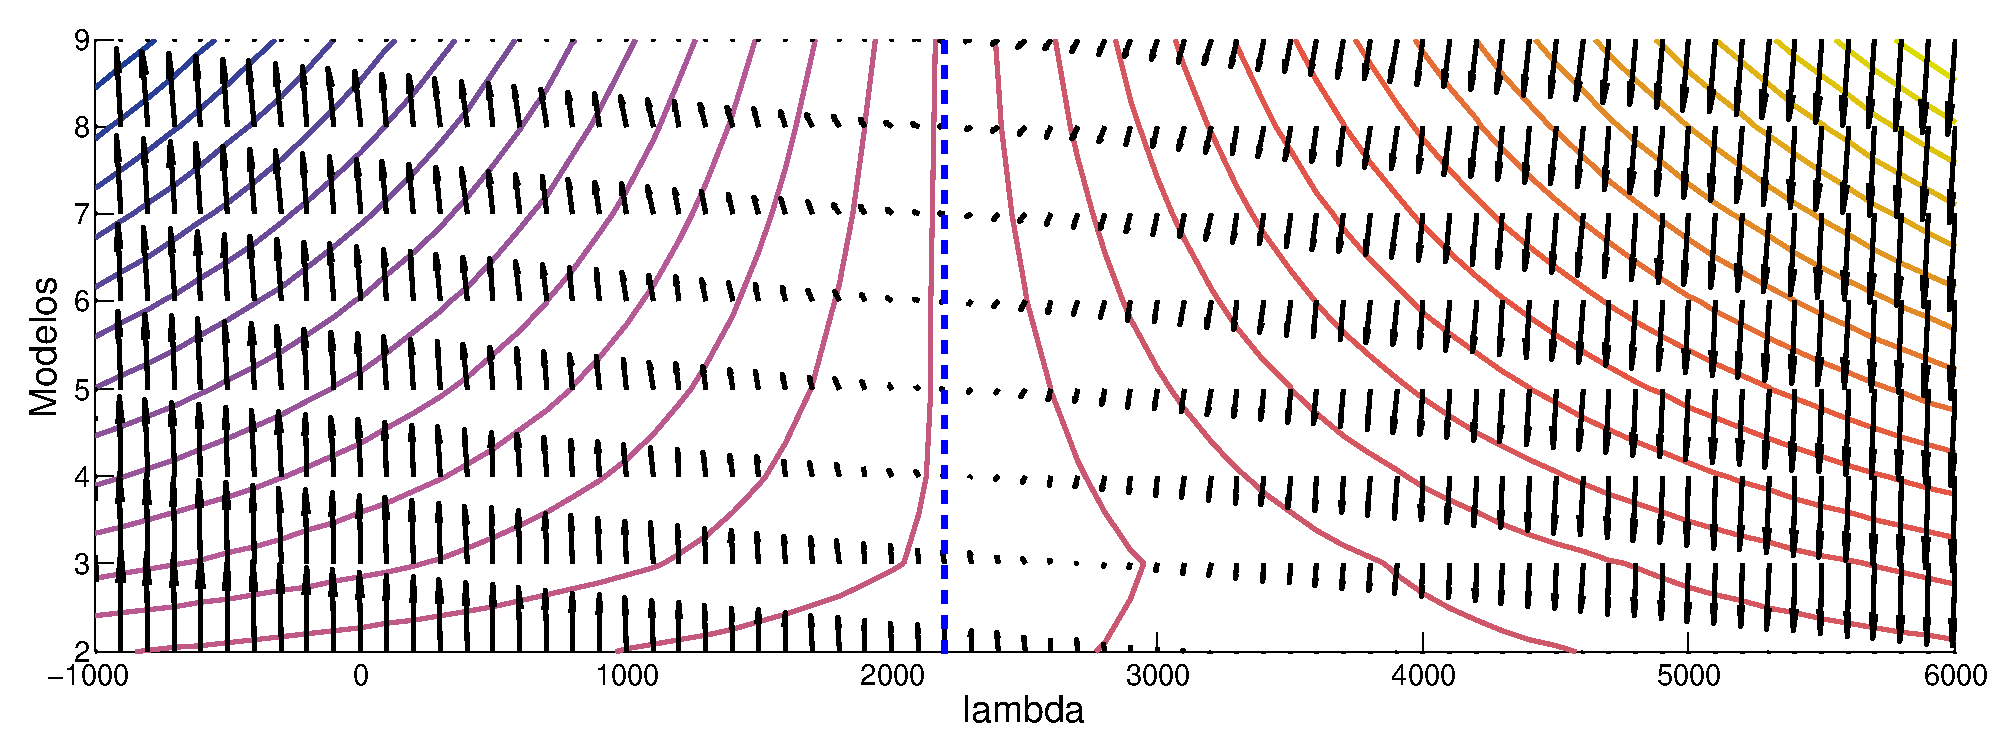
\includegraphics[width=1\textwidth]{gfx/chap6/calderon1bic2}
   \caption{}
   \label{fig:seq2_bic2}
  \end{subfigure}  
  }  
  \centerline{
  \begin{subfigure}[b]{0.55\textwidth}
    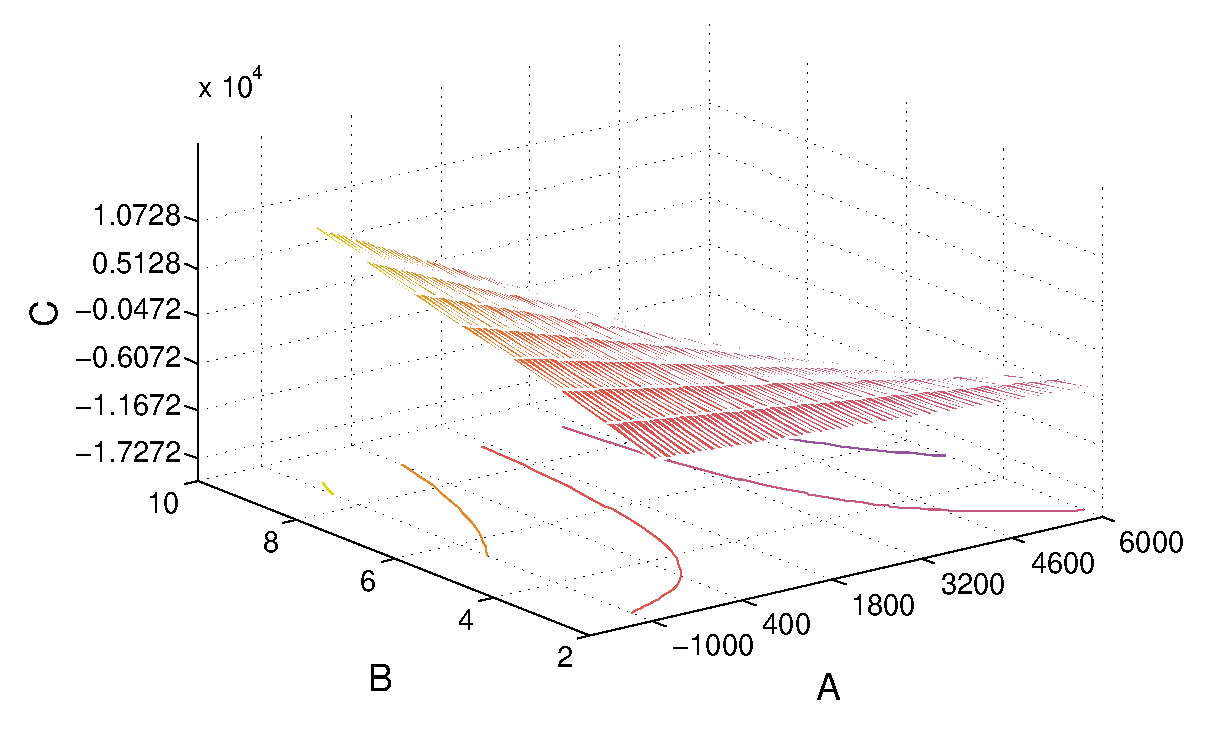
\includegraphics[width=\textwidth]{gfx/chap6/calderon1bic1} 
    \caption{}
    \label{fig:seq2_bic1}
  \end{subfigure}  
  \begin{subfigure}[b]{0.55\textwidth}
    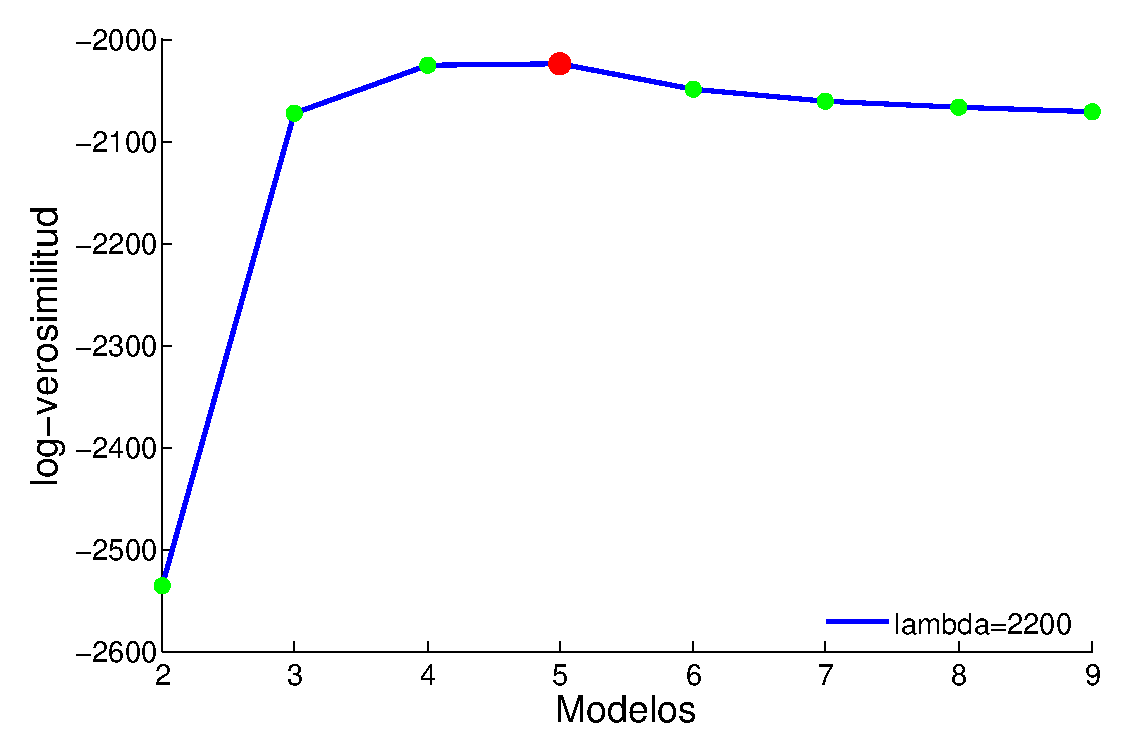
\includegraphics[width=\textwidth]{gfx/chap6/calderon1bic3} 
    \caption{}
    \label{fig:seq2_bic3}
  \end{subfigure}
  }
  \caption[Secuencia 2: Pruebas BIC]{En la \autoref{fig:seq2_bic2}, se muestra las curvas de nivel de la superficie al variar el valor de lambda para evaluar BIC, así como la dirección del gradiente en la misma. En la \autoref{fig:seq2_bic1} se muestra una perspectiva general de superficie en \autoref{fig:seq2_bic2}. En la \autoref{fig:seq2_bic3} se muestra el valor seleccionado para lambda de acuerdo al análisis de sensibilidad realizado en la superficie anterior.}
  \label{fig:seq2_bic}
\end{figure}

En la \autoref{fig:seq2_bic1} se muestra la superficie generada al variar el valor de $\lambda$ para diferentes curvas de selección \ac{BIC}. Haciendo un análisis de sensibilidad se puede determinar cuál es el parámetro $\lambda$ adecuado que penaliza de buena forma la log-verosimilitud. En la \autoref{fig:seq2_bic2} se muestran las curvas de nivel de la figura anterior, además de la dirección del gradiente de la misma. Así mismo, en falso color se resaltan las zonas en las que el gradiente es menor. 

Por último, se muestra en \autoref{fig:seq2_bic3} la curva \ac{BIC} con el valor de $\lambda$ encontrado a partir del análisis de sensibilidad realizado en la \autoref{fig:seq2_bic2}. El o los modelos que tengan un mayor valor \ac{BIC} serán los que se seleccionarán como modelos ganadores.

\begin{figure}[t!]
  \centerline  
  { \begin{subfigure}[b]{0.7\textwidth}
      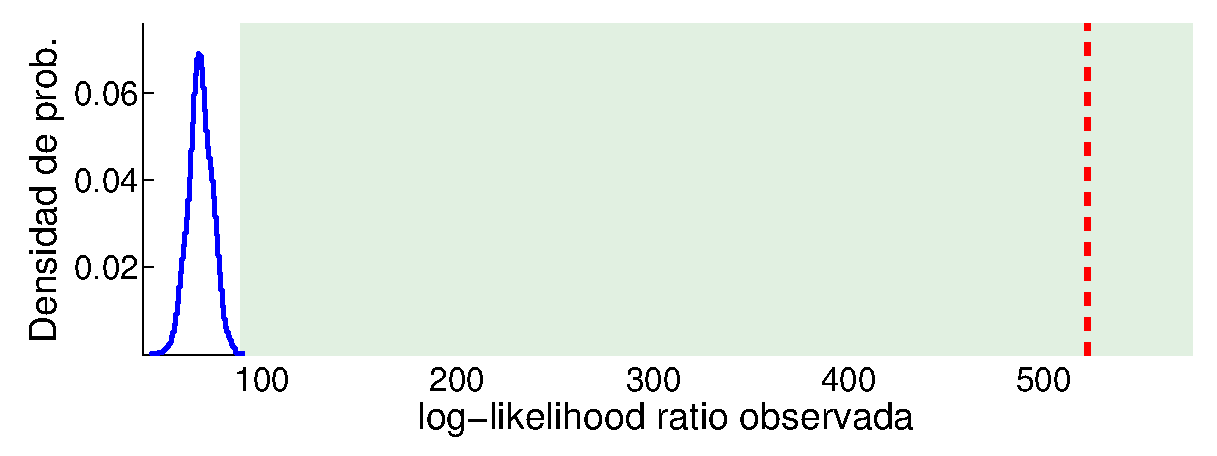
\includegraphics[width=1\linewidth]{gfx/chap6/soledad1boot1}
      \caption{}
      \label{fig:seq2_boot1}
    \end{subfigure}
    \hspace{0.5cm}
    \begin{subfigure}[b]{0.7\textwidth}
      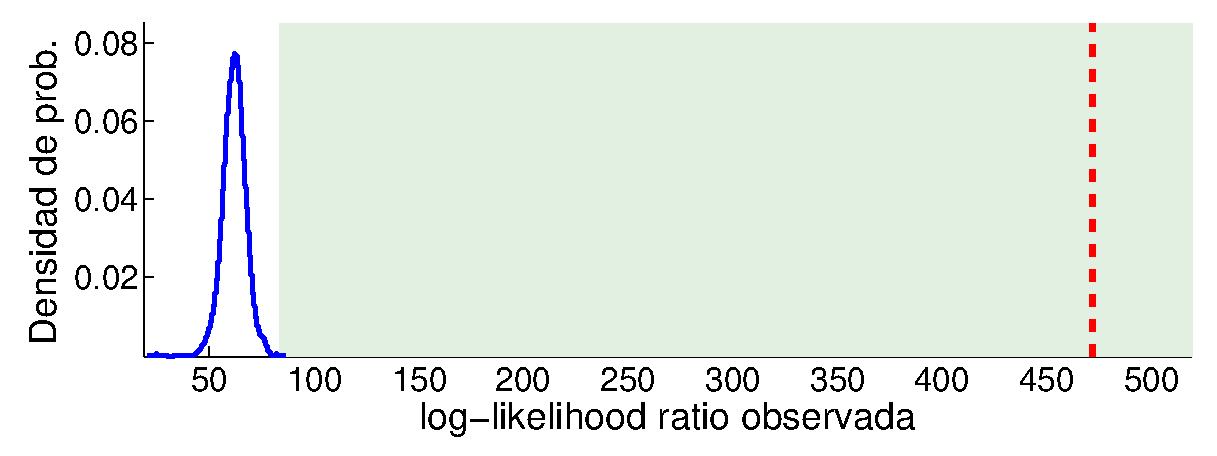
\includegraphics[width=1\linewidth]{gfx/chap6/soledad1boot2}
      \caption{}
      \label{fig:seq2_boot2}
    \end{subfigure}
  }
  \centerline  
  { \begin{subfigure}[b]{0.7\textwidth}
      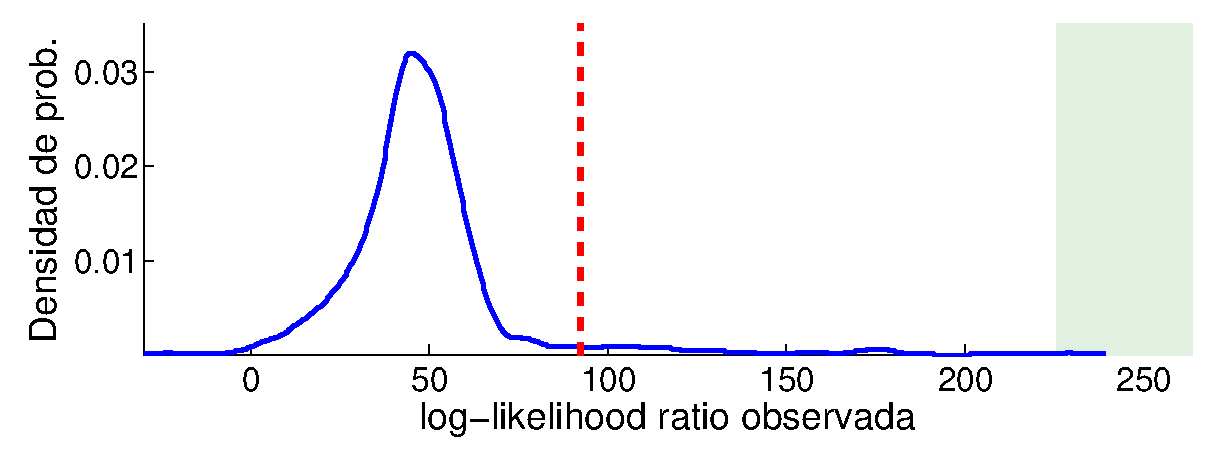
\includegraphics[width=1\linewidth]{gfx/chap6/soledad1boot3}
      \caption{}
      \label{fig:seq2_boot3}
    \end{subfigure}
    \hspace{0.5cm}
    \begin{subfigure}[b]{0.7\textwidth}
      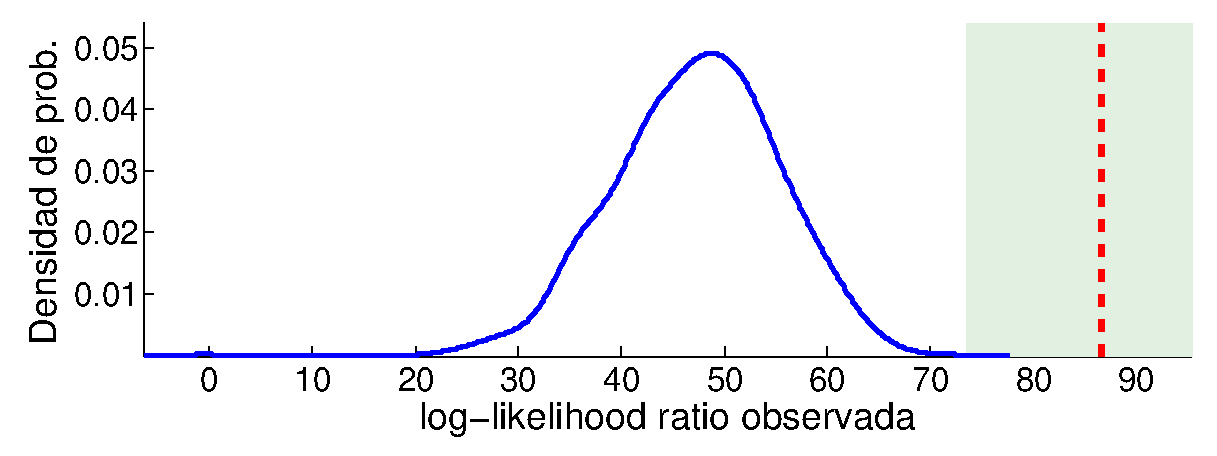
\includegraphics[width=1\linewidth]{gfx/chap6/soledad1boot4}
      \caption{}
      \label{fig:seq2_boot4}
    \end{subfigure}
  }
  \caption[Secuencia 2: Pruebas de hipótesis usando bootstrap]{En la \autoref{fig:seq2_boot1} se muestra la prueba de hipótesis realizada para comparar el modelo $n_2$ contra $n_3$. Como se observa, se rechaza la hipótesis de que el modelo correcto sea $n_4$. En la \autoref{fig:seq2_boot2} se hace la prueba del modelo $n_3$ contra $n_4$, y de la misma manera, se rechaza la hipótesis de que el modelo correcto sea $n_3$. Se sigue con la prueba de hipótesis del modelo $n_4$ contra $n_5$ en la \autoref{fig:seq2_boot3}, y en este caso el valor observado no cae dentro de la región de rechazo, por lo que no podemos rechazar que el modelo $n_4$ sea el correcto. Por último en la \autoref{fig:seq2_boot4}, se hace la prueba del modelo $n_5$ contra el modelo $n_6$, y se vuelve a rechazar la hipótesis nula.}  
  \label{fig:seq2_boot}
\end{figure}

En caso de que después de utilizar BIC se presente ambigüedad para determinar un modelo ganador, o ya sea para realizar un análisis más exhaustivo, se puede propone hacer una prueba de hipótesis para determinar cuál modelo se ajusta mejor a los datos.

A diferencia de la primer etapa, en la que se usa BIC como criterio para  seleccionar el mejor modelo de un conjunto no definido de modelos con diferentes parámetros, la intención de hacer pruebas de hipótesis es determinar en un pequeño conjunto de probables modelos, cuál es mejor, y qué tan bueno es un modelo respecto a otro.

Al plantear la prueba de hipótesis se harán una gran cantidad de simulaciones para ver qué tan bien se ajusta cada modelo a los datos originales, por lo que este proceso es computacionalmente intensivo y sólo se recomienda hacerlo para evitar la ambigüedad entre un par de modelos.

...

Por último, ya con el modelo seleccionado, se procede a calcular el error relativo de predicción que se obtuvo, comparando con el ground truth que se dispone para esa secuencia, con lo que se obtiene: 

...

\begin{figure}[tp]
  \centerline
  {\begin{subfigure}[b]{1.3\textwidth}
      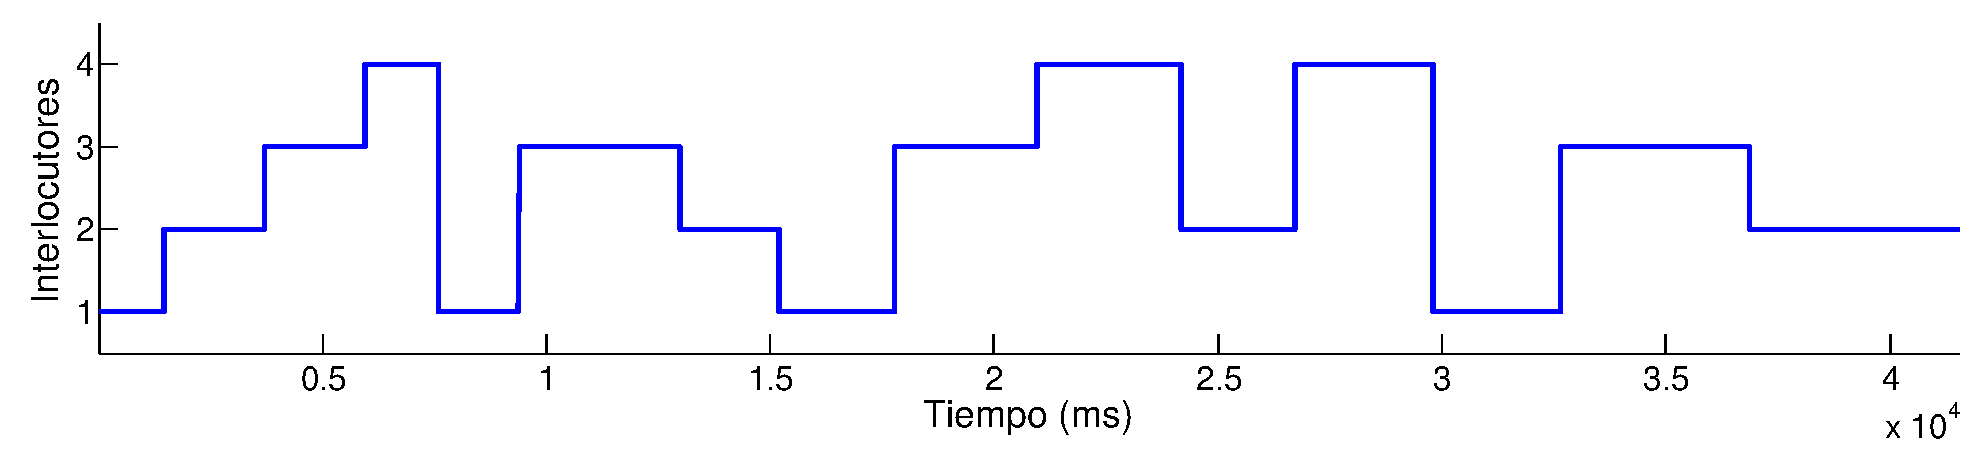
\includegraphics[width=1\linewidth]{gfx/chap6/soledad1s_3_1}
      \caption{}
      \label{fig:seq2_seq1}
    \end{subfigure}
  } 
  \centerline
  {\begin{subfigure}[b]{1.3\textwidth}
      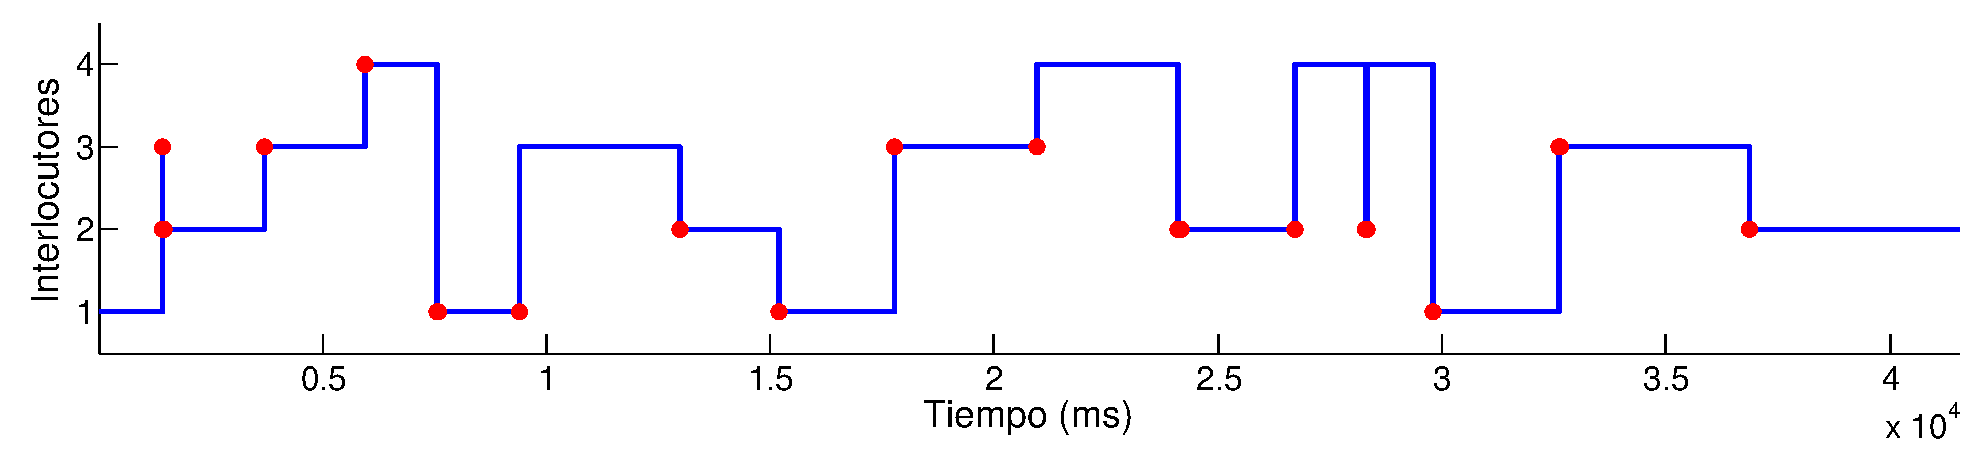
\includegraphics[width=1\linewidth]{gfx/chap6/soledad1s_3_2}
      \caption{}
      \label{fig:seq2_seq2}
    \end{subfigure}
  }
  \caption[Secuencia 2: Secuencia recuperada]{En \autoref{fig:seq2_seq1} se muestra la secuencia original de la \autoref{ssub:soledad}. En comparación, en \autoref{fig:seq2_seq2} se muestra la secuencia recuperada del modelo ganador y se marcan en rojo los errores cometidos respecto a la primera secuencia. }
  \label{fig:prb2_seq}
\end{figure}

Más a detalle, en la \autoref{fig:prb2_seq} se observa en azul el orden en el que participan los interlocutores de acuerdo a la secuencia recuperada. En rojo se marcan tanto los falsos positivos como los falsos negativos, de acuerdo al ground truth. Hay que notar que cuando el número de estados para un modelo no es el correcto, entonces inminentemente el número de errores en la secuencia obtenida será mayor, pues al menos todas las intervenciones de un hablante no podrán ser emparejadas o serán asignadas a alguien más.

Se observa también que la mayoría de las veces, en la secuencia recuperada se encuentran algunos brincos entre personas, pero en esencia la estructura y el orden en que hablan los interlocutores es el correcto.